\documentclass[]{article}
\usepackage{lmodern}
\usepackage{amssymb,amsmath}
\usepackage{ifxetex,ifluatex}
\usepackage{fixltx2e} % provides \textsubscript
\ifnum 0\ifxetex 1\fi\ifluatex 1\fi=0 % if pdftex
  \usepackage[T1]{fontenc}
  \usepackage[utf8]{inputenc}
\else % if luatex or xelatex
  \ifxetex
    \usepackage{mathspec}
  \else
    \usepackage{fontspec}
  \fi
  \defaultfontfeatures{Ligatures=TeX,Scale=MatchLowercase}
\fi
% use upquote if available, for straight quotes in verbatim environments
\IfFileExists{upquote.sty}{\usepackage{upquote}}{}
% use microtype if available
\IfFileExists{microtype.sty}{%
\usepackage{microtype}
\UseMicrotypeSet[protrusion]{basicmath} % disable protrusion for tt fonts
}{}
\usepackage[margin=1in]{geometry}
\usepackage{hyperref}
\hypersetup{unicode=true,
            pdftitle={BMI702 Final Project Report},
            pdfauthor={Niklas Rindtorff},
            pdfborder={0 0 0},
            breaklinks=true}
\urlstyle{same}  % don't use monospace font for urls
\usepackage{graphicx,grffile}
\makeatletter
\def\maxwidth{\ifdim\Gin@nat@width>\linewidth\linewidth\else\Gin@nat@width\fi}
\def\maxheight{\ifdim\Gin@nat@height>\textheight\textheight\else\Gin@nat@height\fi}
\makeatother
% Scale images if necessary, so that they will not overflow the page
% margins by default, and it is still possible to overwrite the defaults
% using explicit options in \includegraphics[width, height, ...]{}
\setkeys{Gin}{width=\maxwidth,height=\maxheight,keepaspectratio}
\IfFileExists{parskip.sty}{%
\usepackage{parskip}
}{% else
\setlength{\parindent}{0pt}
\setlength{\parskip}{6pt plus 2pt minus 1pt}
}
\setlength{\emergencystretch}{3em}  % prevent overfull lines
\providecommand{\tightlist}{%
  \setlength{\itemsep}{0pt}\setlength{\parskip}{0pt}}
\setcounter{secnumdepth}{0}
% Redefines (sub)paragraphs to behave more like sections
\ifx\paragraph\undefined\else
\let\oldparagraph\paragraph
\renewcommand{\paragraph}[1]{\oldparagraph{#1}\mbox{}}
\fi
\ifx\subparagraph\undefined\else
\let\oldsubparagraph\subparagraph
\renewcommand{\subparagraph}[1]{\oldsubparagraph{#1}\mbox{}}
\fi

%%% Use protect on footnotes to avoid problems with footnotes in titles
\let\rmarkdownfootnote\footnote%
\def\footnote{\protect\rmarkdownfootnote}

%%% Change title format to be more compact
\usepackage{titling}

% Create subtitle command for use in maketitle
\providecommand{\subtitle}[1]{
  \posttitle{
    \begin{center}\large#1\end{center}
    }
}

\setlength{\droptitle}{-2em}

  \title{BMI702 Final Project Report}
    \pretitle{\vspace{\droptitle}\centering\huge}
  \posttitle{\par}
    \author{Niklas Rindtorff}
    \preauthor{\centering\large\emph}
  \postauthor{\par}
      \predate{\centering\large\emph}
  \postdate{\par}
    \date{4/15/2019}


\begin{document}
\maketitle

\hypertarget{final-project}{%
\section{Final Project}\label{final-project}}

\hypertarget{introduction}{%
\subsection{Introduction}\label{introduction}}

Cancer is an extremely heterogenous disease. While the availability of
genomic testing of tumors is continously increasing, linking the correct
drug to the right patient remains a challenge. Part of this challenge is
the difficulty to predict drug responses to a large number of drugs
based on a tumors genetic profile.

In order to increase our understanding of how genetic markers predict
drug response, laboratory tumor models, such as 2D cancer cell lines,
can be treated with a large number of therapeutics in-vitro. The drug
response of these tumor models, in combination with their genetic data,
can then be associated.

\hypertarget{part-1-the-cancerrxgene-dataset}{%
\subsection{Part 1: The CancerRxGene
Dataset}\label{part-1-the-cancerrxgene-dataset}}

In this project I present the
\href{https://www.cancerrxgene.org/translation/Drug/179\#vp}{\textbf{CancerRxGene
Dataset}} by the Genomics in Drug Sensitivity in Cancer Project. It
contains genomic information for \textgreater{}1000 cancer cell lines
together with in-vitro drug response information. The data can be used
to find genomic biomarkers of drug response in cancer cell lines. In the
future, this dataset will be maintained by the DepMap project, a joint
effort by the Wellcome Trust Sanger Institute and the Broad Institute.
The data is publicly available. To the best of my knowledge, it is one
of the greates non-commercial drug sensitivity datasets in cancer
models.

\begin{figure}
\centering
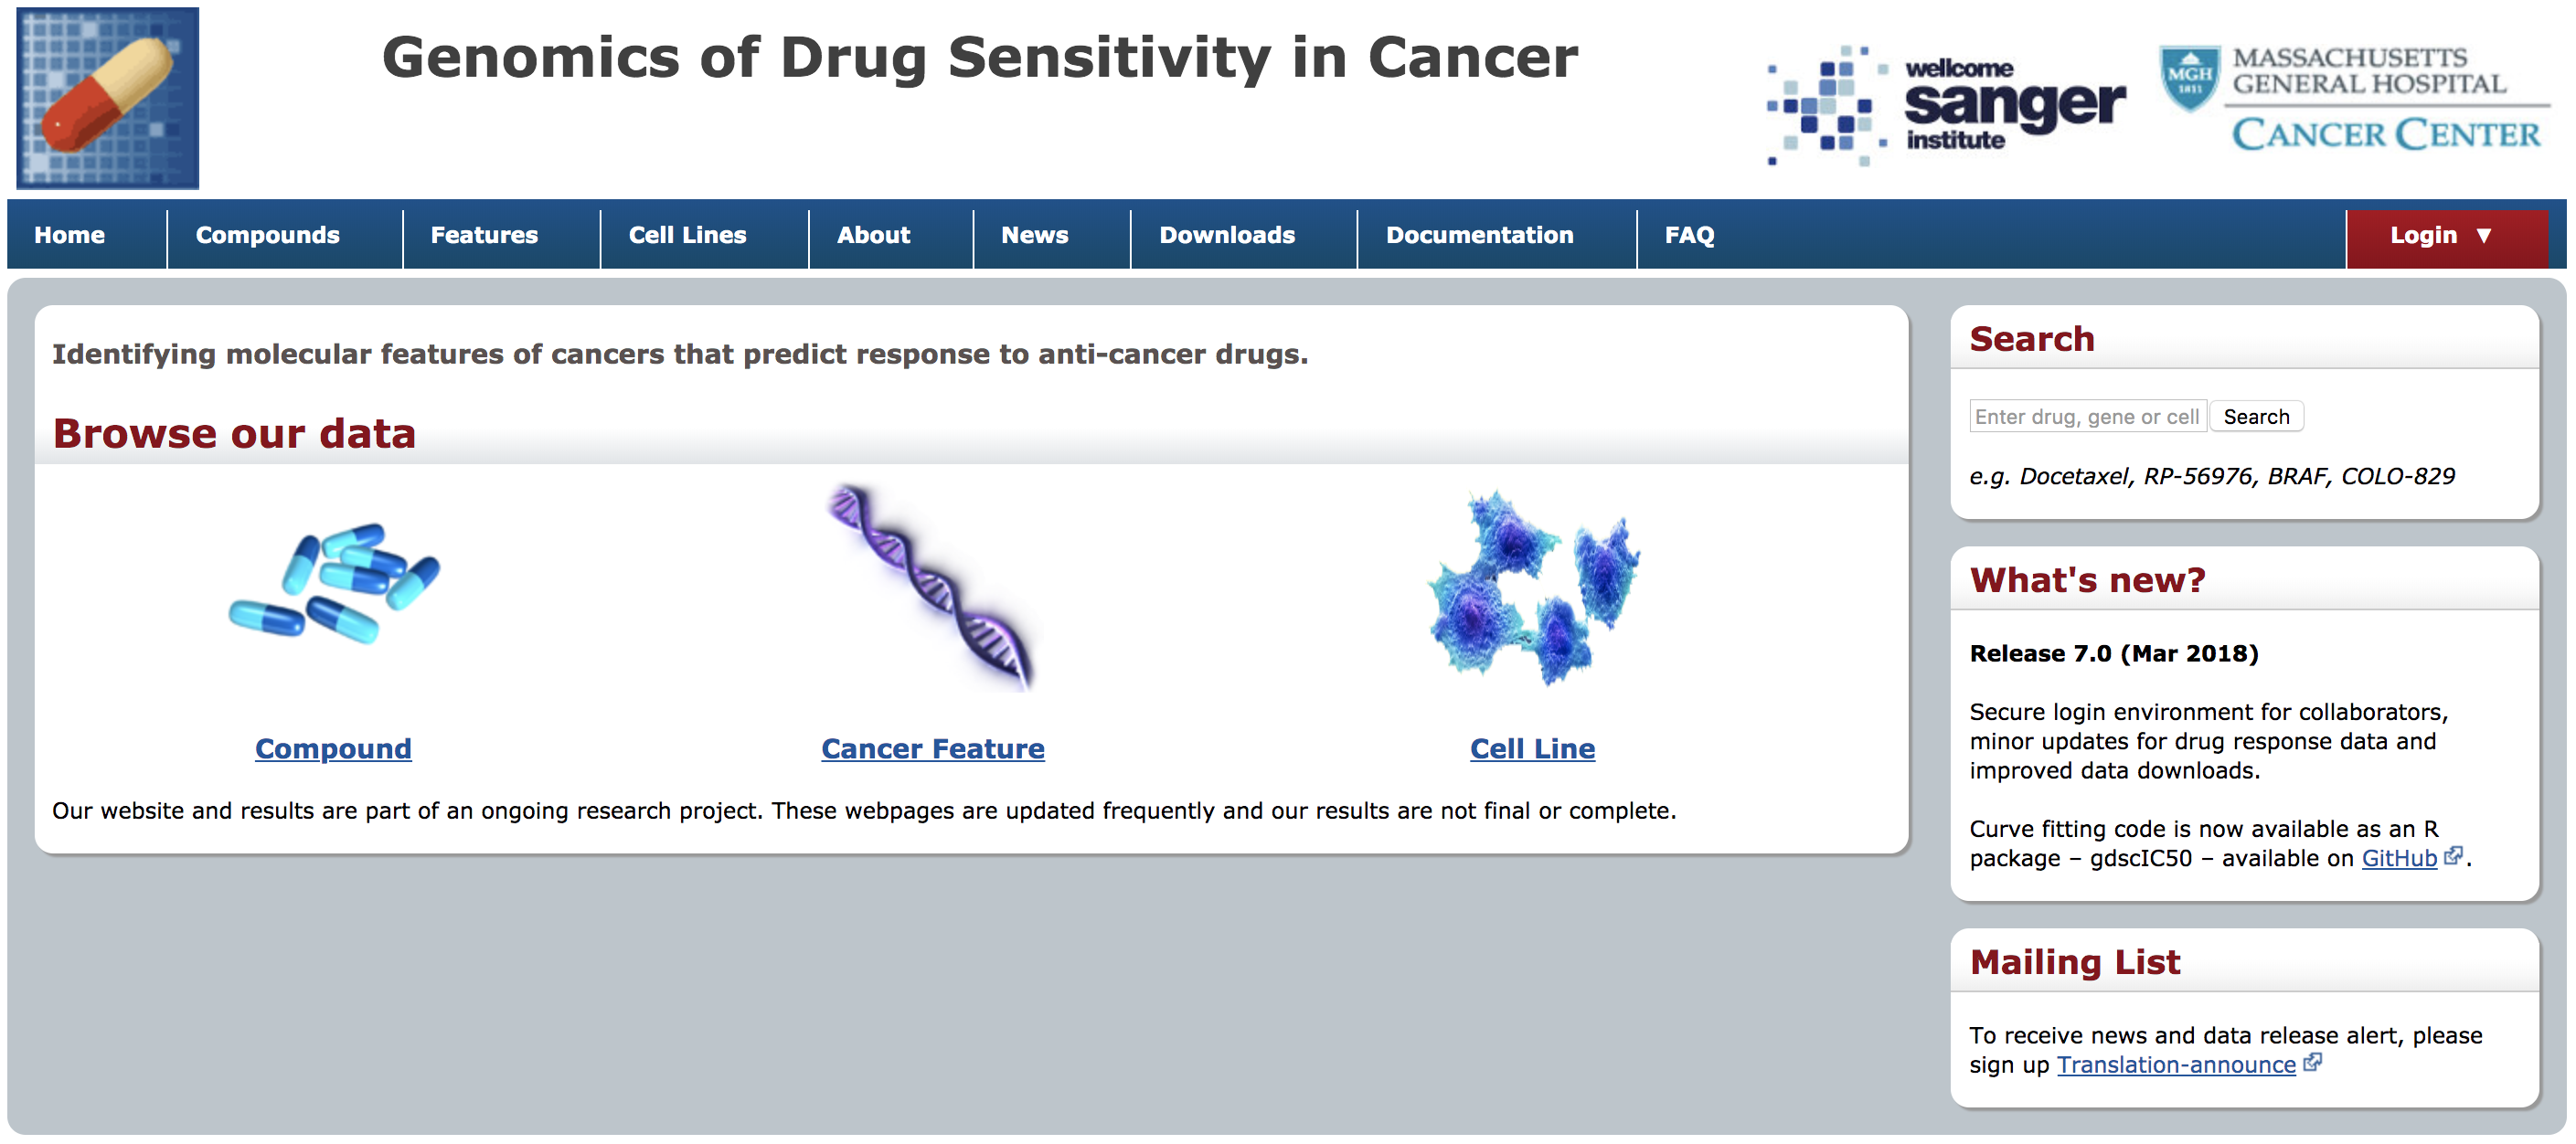
\includegraphics{landing_page.png}
\caption{Landing page of the CancerRxGene Portal}
\end{figure}

\textbf{Who publishes the dataset?} The data is published by the
Genomics in Drug Sensitivity in Cancer Project. The project is a joint
effort by the Cancer Genome Project, the Wellcome Trust Sanger institute
and the Center for Molecular Therapeutics at MGH.

\textbf{Why do they publish it?} The data is funded by public
entitities, such as the Wellcome Trust and is published in scientific
publications. To increase the access of the project's data, the data is
freely available online.

\textbf{How frequently is it updated?} The data is updated in an
irregular schedule, when a batch of cancer cell line vulnerability data
has been collected and pre-processed. The last update of the dataset was
published in March 2018.

\textbf{What variables does it contain?} The dataset contains multiple
tables: * meta-data about every cancer cell line, such as culture medium
and tissue of origin. * copy-number variants for every cell line, in the
form of a binary matrix * gene expression data for every cell line, in
the form of a numeric matrix * drug response data for every cell line.
The data contains \emph{IC50} values for \textgreater{}60 drugs.

\textbf{How is it delivered?} The data is available on the project's
\href{https://www.cancerrxgene.org/downloads}{website} and is split
across multiple Excel files.

\textbf{Are there any restrictions on its use or availability?} Yes, the
data is subject to restrictions: \emph{``Users have a non-exclusive,
non-transferable right to use data files for internal, non-commercial
research and educational purposes Please note: The data files are
experimental and academic in nature and are not licensed or certified by
any regulatory body. Genome Research Limited provides access to data
files on an ``as is'' basis and excludes all warranties of any kind
(express or implied)."}.

\textbf{Does it make use of any standard (or proprietary) ontologies or
terminologies?} The data uses \emph{COSMIC IDs} to identify cell lines.
The gene expression data is annotated using the
\href{https://useast.ensembl.org/index.html}{Ensemble} nomenclature. The
gene mutation dataset is annotated using the \emph{HUGO} terminology.
The drugs tested are not linked to a standardized ontology.

\textbf{What are some questions that have been asked previously using
the data?} Previously, this data has been used to find predictive models
that link genetic markers with drug response
\href{https://www.cell.com/fulltext/S0092-8674(16)30746-2}{Iorio et al.,
2016}. In addition visualization projects have created
\href{https://journals.plos.org/plosone/article?id=10.1371/journal.pone.0176763}{applications}
to explore this dataset.

\begin{figure}
\centering
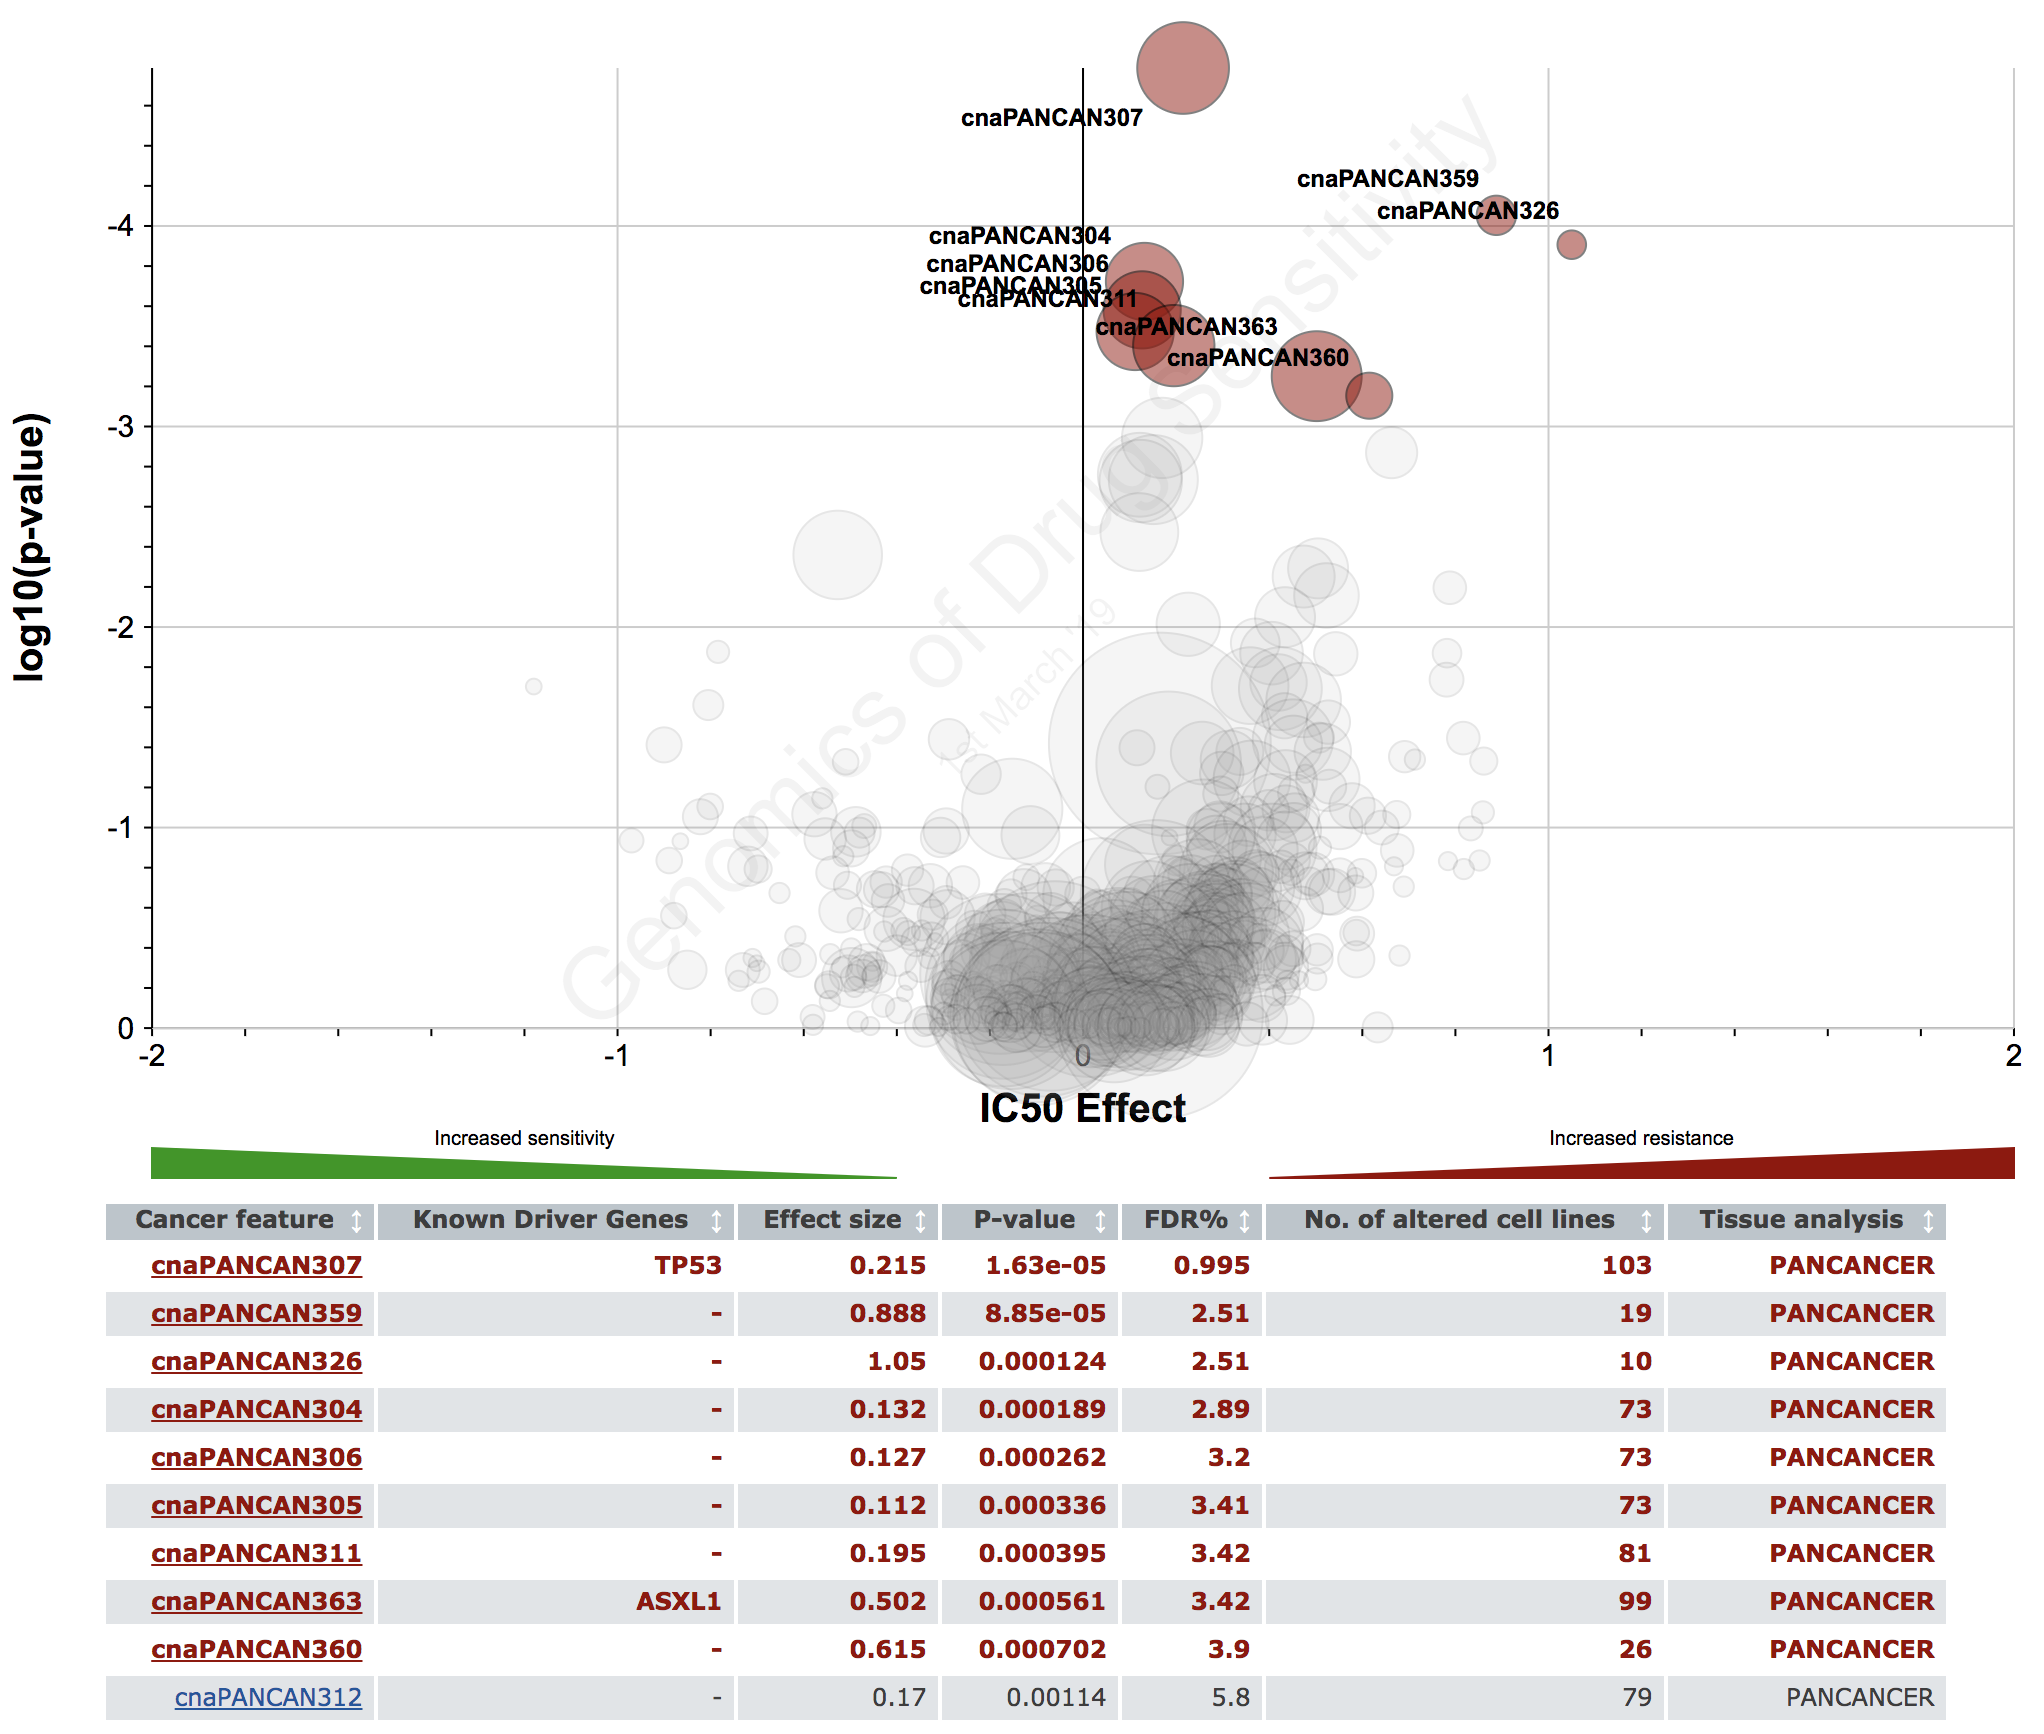
\includegraphics{vulcano.png}
\caption{Examplatory analysis in the CancerRxGene Portal: Which genomic
features are associated with drug sensitivity to the chemotherapeutic
5-FU}
\end{figure}

\newpage

\hypertarget{part-2-identification-of-potential-personalized-cancer-combination-therapies-under-a-non-synergy-assumption}{%
\subsection{Part 2: Identification of potential personalized cancer
combination therapies under a non-synergy
assumption}\label{part-2-identification-of-potential-personalized-cancer-combination-therapies-under-a-non-synergy-assumption}}

\hypertarget{introduction-1}{%
\subsubsection{Introduction}\label{introduction-1}}

\begin{figure}
\centering
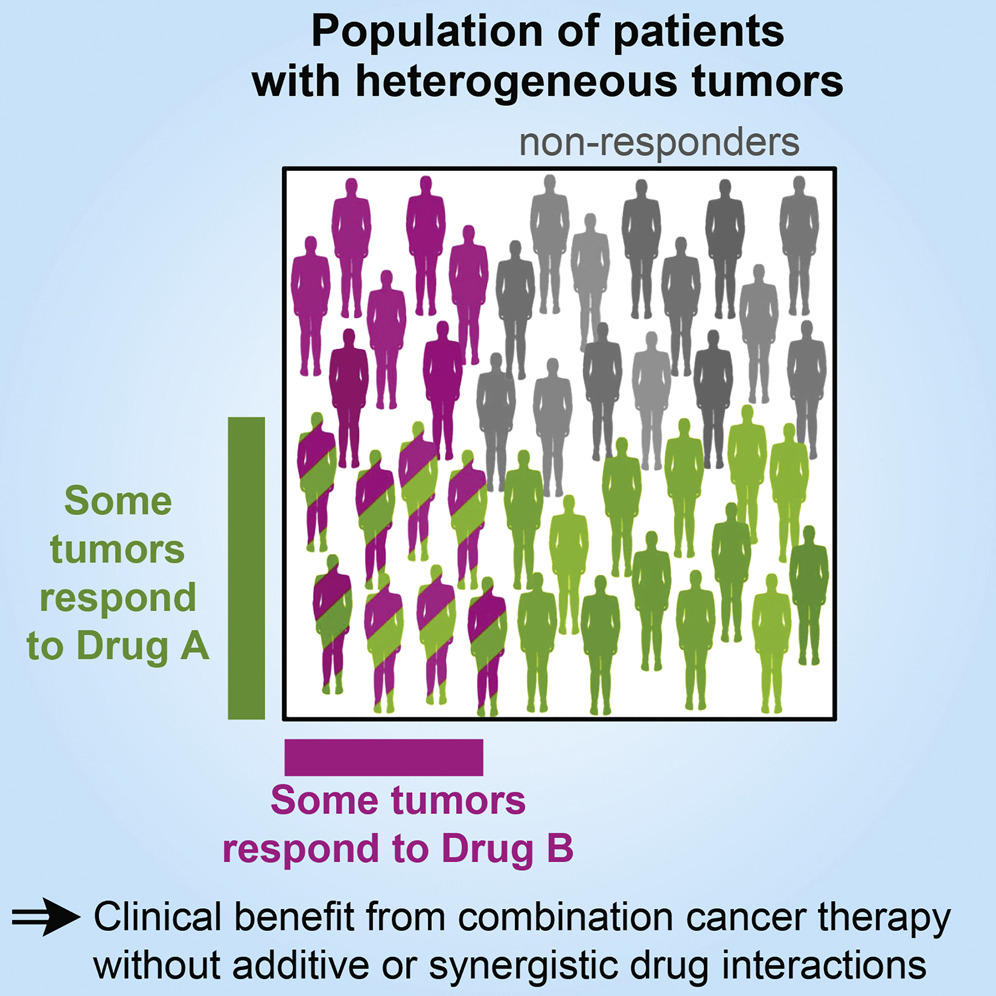
\includegraphics{vis_abstract.jpg}
\caption{Visual Abstract of \emph{Combination Cancer Therapy Can Confer
Benefit via Patient-to-Patient Variability without Drug Additivity or
Synergy} by Palmer et al.}
\end{figure}

I downloaded the respective tables and preprocessed the drug response
data by log transforming and median centering IC50 values for each drug
over every cell line. By transforming IC50 values this way, we can
compare drug effects between both cell lines and drugs.

\begin{figure}
\centering
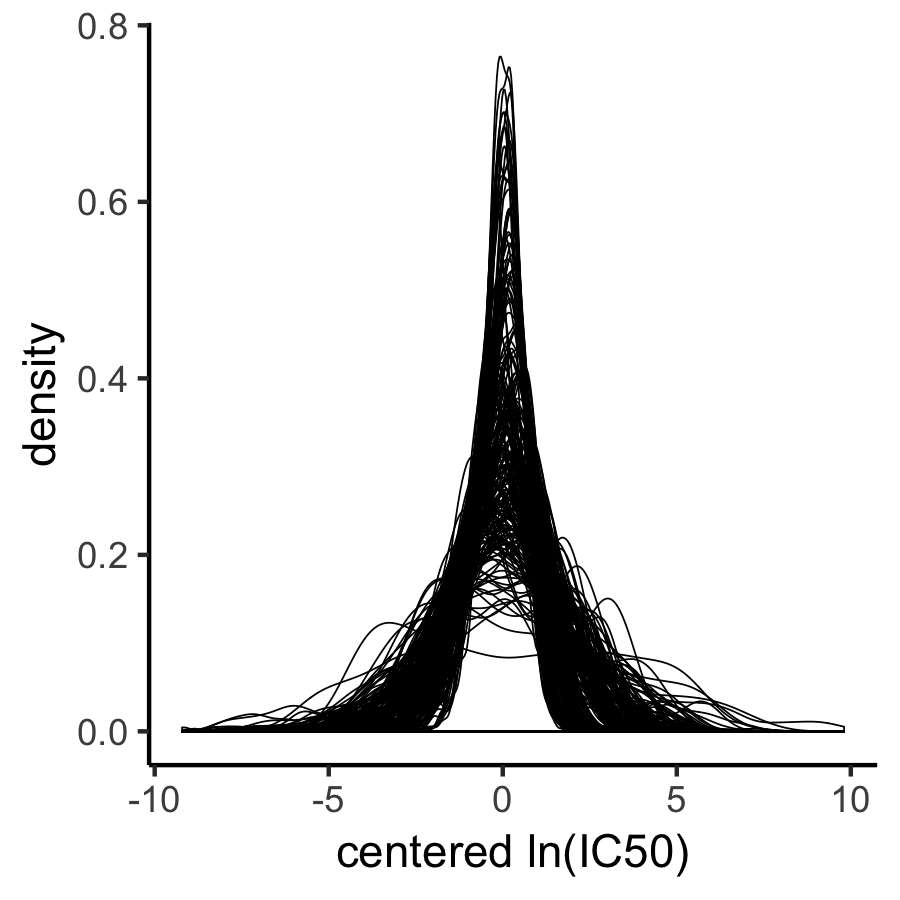
\includegraphics{center_ic50.png}
\caption{Distribution of log(IC50) values after centering}
\end{figure}

Prior studies in mouse models of epithelial cancers suggests, that the
main driver of superiority of combination cancer therapy over
single-agent regimen is not biochemical synergy between agents, but an
increased probability of either one of the agents causing a therapeutic
effect in a patient's disease. According to this theory, combination
treatments with agents that have anti-correlated response profiles are
interesting candidate compounds for further clinical evaluation. In
their original study the authors demonstrate that in fact the majority
of currently administred combination treatments in oncology are not
positiviely correlated.

In this study, my goal is to identify new potential combinations of
therapeutics that are anticorrelated. Because oncology today is a highly
specialized field, it is not sufficient to only identify compounds that
are anti-correlated from a pan-cancer perspective. Instead, I will run
multiple correlation analysis on subsets of cancer cell lines defined by
tissue of origin or mutation status. Because, the estimation of
correlation coefficients is not stable with differing number of samples
and subsetting of the dataset leads to very small subgroups, I have to
introduce methods to estimate the credible intervals of correlation
coefficients.

\begin{figure}
\centering
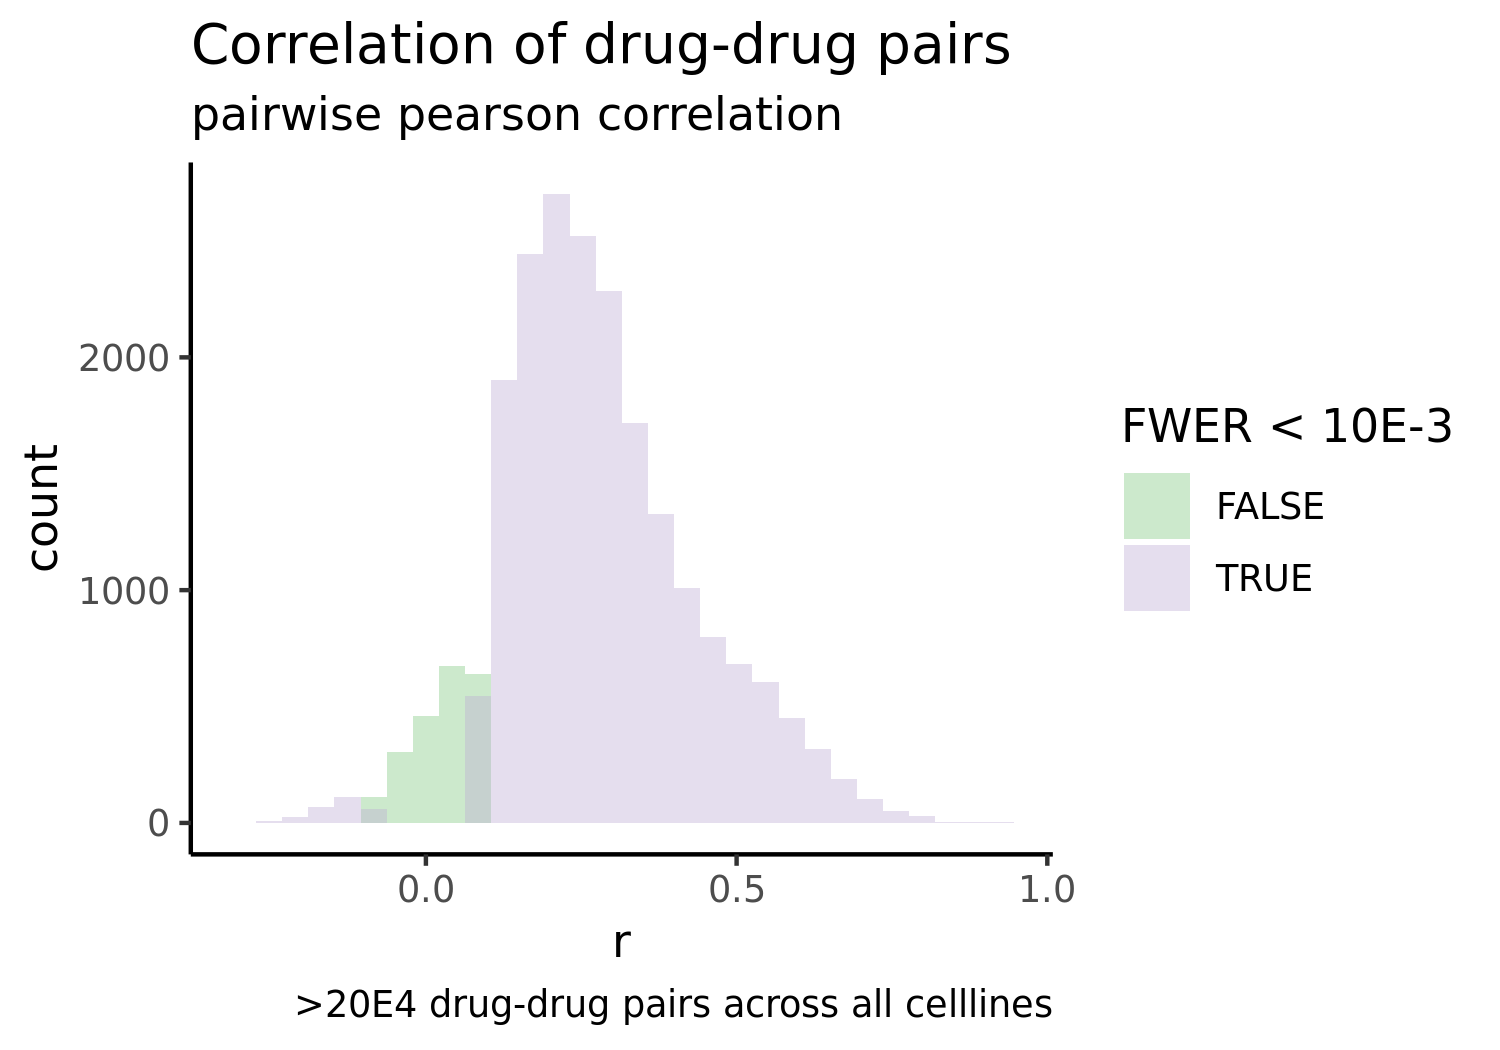
\includegraphics{pan_cancer_r_hist.png}
\caption{Correlation of drug-drug pairs across all possible combinations
using all available cellline models}
\end{figure}

\#{[}Increased variance of correlation coefficients as subgroup size
decreases{]}

Visualize key variables Use a supervised or unsupervised machine
learning method to explore a question Do (at least) one of the
following: Load the data into a relational database management system
Use NLP to analyze part of the data Build an app that helps other people
explore the data Some other extension (discuss with Adam)

Part 3:


\end{document}
